% Это основная команда, с которой начинается любой \LaTeX-файл. Она отвечает за тип документа, с которым связаны основные правил оформления текста.
\documentclass{article}[a4paper, 14pt]

% Здесь идет преамбула документа, тут пишутся команды, которые настраивают LaTeX окружение, подключаете внешние пакеты, определяете свои команды и окружения. В данном случае я это делаю в отдельных файлах, а тут подключаю эти файлы.

% Здесь я подключаю разные стилевые пакеты. Например возможности набирать особые символы или возможность компилировать русский текст. Подробное описание внутри.
\usepackage{packages}

% Здесь я определяю разные окружения, например, теоремы, определения, замечания и так далее. У этих окружений разные стили оформления, кроме того, эти окружения могут быть нумерованными или нет. Все подробно объяснено внутри.
\usepackage{environments}

% Здесь я определяю разные команды, которых нет в LaTeX, но мне нужны, например, команда \tr для обозначения следа матрицы. Или я переопределяю LaTeX команды, которые работают не так, как мне хотелось бы. Типичный пример мнимая и вещественная часть комплексного числа \Im, \Re. В оригинале они выглядят не так, как мы привыкли. Кроме того, \Im еще используется и для обозначения образа линейного отображения. Подробнее описано внутри.
\usepackage{commands}

% Пакет для титульника проекта
\usepackage{titlepage}

% Пакеты для отображения картинок
\usepackage{graphicx}
\usepackage{float}
\usepackage{wrapfig}

%
%\usepackage[unicode=true, colorlinks=true, linkcolor=blue, urlcolor=blue]{hyperref}


% Здесь задаем параметры титульной страницы
\setUDK{192.168.1.1}
% Выбрать одно из двух
%\setToResearch
%\setToProgram
\setToPractice

\setTitle{Мобильное приложение для отслеживания привычек}


\setStageOne

%сюда можно воткнуть картинку подписи
\setStudentSgn{}

\providecommand{\studentCompleted}{Выполнил студент}
\providecommand{\student}{TestStudent}
\providecommand{\group}{404}

\setStudent{\student}
\setGroup{\group}

\setStudentDate{20.10.2022}
\setAdvisor{Колесниченко Елена Юрьевна}
\setAdvisorTitle{департамент больших данных и информационного поиска ФКН ВШЭ, доцент}
\setAdvisorAffiliation{ООО <<Яндекс. Технологии>>}
\setAdvisorDate{24.10.2022}
\setGrade{--}
%сюда можно воткнуть картинку подписи
% \setAdvisorSgn{\scalebox{0.4}{\includegraphics{Utils/advisor_sign}}}
\setYear{2022}

\setStudentCompleted{\studentCompleted}

\linespread{1.2}
\urlstyle{same}

\bibliographystyle{Bibliography/gost-numeric.bbx}
\usepackage[parentracker=true,
backend=biber,
hyperref=true,
bibencoding=utf8,
language=auto,
autolang=other,
citestyle=gost-numeric,
defernumbers=true,
bibstyle=gost-numeric,
sorting=ntvy,
maxbibnames=99,
]{biblatex}

\addbibresource{Bibliography/sources.bib}

\setlength{\parskip}{6pt}
\setlength{\parindent}{10pt}

% С этого момента начинается текст документа
\begin{document}

% Эта команда создает титульную страницу
% \makeTitlePage

\newpage 


\vspace*{\fill}

\begin{center}
    \huge
    План выполнения курсовой работы по теме \\
    <<Реализация поддержки асинхронного программирования для фреймворка DSLab>>
\end{center}
    
\vspace*{\fill}

\newpage

% Здесь будет автоматически генерироваться содержание документа
\tableofcontents


\newpage
%!TEX root=../main.tex


\section*{Аннотация}

DSLab - программный фреймворк для имитационного моделирования и тестирования распределенных систем.

В проекте используется дискретно-событийный подход описания моделей и приложений, где события обрабатываются в пользовательских функциях (callback-ах). В рамках проекта предстоит добавить возможность управлять событиями асинхронно.


\section{Описание проекта и постановка задачи}

\subsection{Устройство DSLab}

В силу широты охвата областей применения фреймворка он организован в виде набора слабо связанных программных модулей, использование которых будет осуществляться через их API. Это даст возможность пользователям фреймворка (исследователям, разработчикам, преподавателям) гибким образом собирать из модулей решения под свои цели, например симуляторы для конкретных типов систем или постановок задач.

Входящие в состав фреймворка модули можно условно разделить на три типа:
\begin{enumerate}
    \item 
    Базовые, функциональность которых используется остальными модулями (например, реализация дискретно-событийного моделирования)
    \item
    Универсальные, функциональность которых может быть использована в различных предметных областях (например, модели сети);
    \item
    Специализированные, которые заточены под определенную предметную область (например, библиотеки для моделирования облачных инфраструктур, исследования алгоритмов планирования заданий на кластерах или тестирования решений учебных заданий).
\end{enumerate}

Архитектуру DSLab можно схематично представить в виде трех слоев (Рис. \ref{dslab_arc}), включающих модули соответствующего типа. На рисунке также указаны текущие модули и зависимости между ними. Зависимости от dslab-core (от него зависят все имеющиеся универсальные и специализированные модули) не указаны, чтобы не загромождать рисунок. Таким образом, модули могут зависеть от модулей с нижних слоев, но не наоборот.

\begin{figure}[H]
    \centering
    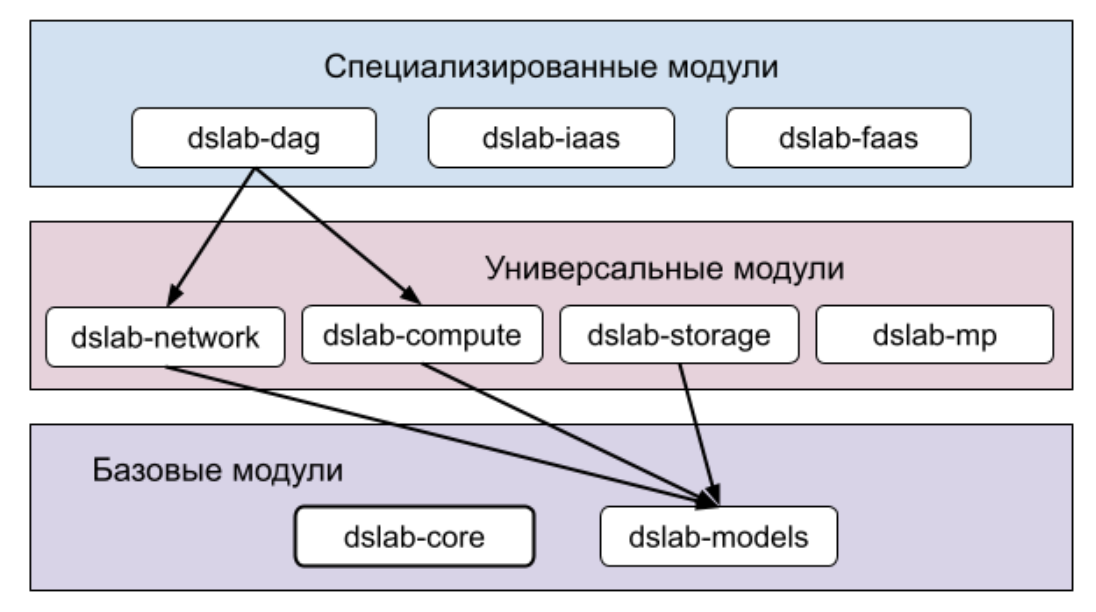
\includegraphics[width=0.7\linewidth]{images/dslab_arc.png}
    \caption{Архитектура DSLab}
    \label{dslab_arc}
\end{figure}


% TODO \cite{dslab-docs}

Таким образом пользователь при разработке собственной симуляции может либо использовать уже готовые разработанные компоненты, либо реализовывать свои и произвольно их связывать. 


Основным процессом создания симуляции является создание событий и написание процессов реагирования на них. Каждое событие представляет из себя следующую структуру: 
\begin{enumerate}
    \item идентификатор события 
    \item идентификатор компонента, создавшего событие 
    \item идентификатор компонента, которому это событие предназначено доставить 
    \item внутреннее время, когда событие должно наступить
    \item произвольные данные события (<<полезная нагрузка>>)
\end{enumerate}

Таким образом в процессе симуляции разные компоненты генерируют события друг для друга и с помощью самого базового модуля dslab-core обмениваются ими. Чтобы как-то реагировать на событие, каждый компонент реализует единственный обобщенный метод \texttt{(trait EventHandler в языке Rust)}, в который dslab-core передает нужное событие. При обработке события компоненты генерируют новые и таким образом цикл симуляции замыкается. 

Получается, что сейчас реагировать на пришедшие события можно только в одном месте -- в той самой функции-callback которую позовет dslab-core. В случае, когда событий немного -- это лаконично выглядит и этим удобно пользоваться. В случае же, если возникает более сложный алгоритм с большим количеством различных событий, и, что важнее, цепочками событий, на которые нужно последовательно реагировать, подобная модель становится не самой удобной. 

Хотелось бы иметь альтернативную возможность писать на языке программирования более понятный с первого взгляда алгоритм, ведь с единой точной входа многие последовательные логичные действия оказываются разбросаны по коду и фрагментированы. 

Как раз такой возможностью является написание асинхронного кода. Тогда какие-то сложные куски логики можно было бы выносить в отдельные функции, держать их вместе, просто исполнение бы прерывалось в ожидании какого-то события, чтобы продолжить.

\subsection{Цель}

Добавить возможность пользователю использовать асинхронность при программировании симуляции в DSLab.

\newpage

\section{Актуальность и значимость}

Как уже было описано в мотивации постановки цели этой работы, главное преимущество асинхронной модели~--~удобство при написании сложных многоступенчатых алгоритмов.

Это так же повысит читаемость кода. Процесс принятия решение о сохранении файла в распределенном хранилище в такой парадигме мог бы выглядеть таким образом (псевдокод):

\begin{lstlisting}[language=Python]
async fn add_file_to_storage(some_file) {
    send_file_to_all_replicas(some_file);
    result = wait_for_confirmation_from_all().await;
    if result.has_quorum {
        send_commit_to_all_replicas();
        wait_for_commit_confirmation_from_quorum().await;
        send_ok_message_to_user();
    } else {
        send_reject_message_to_user();
    }
}
\end{lstlisting}

Посмотрев на функцию можно понять, что она делает, потому что логика последовательна и удобна разбита на подфункции. У нас есть возможность написать такой алгоритм на верхнем уровне, а не обрабатывать сообщения всех типов от всех реплик в одной функции.


\section{Существующие работы и решения}

Подобный подход уже был реализован в других симуляторах, например в \href{https://github.com/osukhoroslov/dslab/blob/main/examples-other/simgrid/ping-pong/process.cpp}
{SimGrid}, но этот код сложно назвать легко читаемым. 

\section{Предлагаемые подходы и методы} 

Чтобы дать возможность пользователю писать асинхронный код, нужно создать саму возможность обрабатывать события асинхронно. Для этого нужно написать свой executor задач в DSLab, который будет исходя из внутренней логики (наступление времени, когда событие нужно доставить получателю) понимать, когда и какую асинхронную задачу нужно разбудить, и дать ей продолжить исполнение. 

Для этого нужно реализовать альтернативу dslab-core (или дополнить уже сущетсвующую реализацию), и затем уже пользоваться новым интерфейсом на более верхних уровнях.

К счастью, язык Rust дает возможность пользователям самим управлять процессом рантайма, поэтому с помощью библиотеки futures подобное поведение может быть реализовано.
% TODO link for crate futures

% TODO link to rust async book

По асинхронному расту есть официальная документация (еще не в завершенном состоянии, но уже достаточно подробная, чтобы начать с нее).

Изучив предлагаемые там примеры и посмотрев материалы был реализован прототип.

% TODO add my link to rust-async-await 

\section{Ожидаемые результаты}

Поддержана возможность реализовывать алгоритмы в DSLab используя асинхронность. В проект добавлены примеры кода, документация по использованию реализованных методов.

\section{План работ}

% TODO link to rust repository shad

\newpage
\addcontentsline{toc}{section}{Список литературы}
\printbibliography

% \addcontentsline{toc}{section}{Список иллюстраций}
% \listoffigures

Требования к DSLab, документация https://docs.google.com/document/d/1CprULnQiVSWTXiBkx90CSEi4tgkUhM3R6VeCp1CsRwo/edit



\end{document}
% Начиная с этого момента весь текст LaTeX игнорирует, можете вставлять любую абракадабру.
